\documentclass[tikz,border=2pt]{standalone}
\usepackage{amsmath}
\usepackage{pgfplots}
\pgfplotsset{compat=1.18}
\usepgfplotslibrary{fillbetween}

\begin{document}
% Signed area: the integral of sin x over [0, 4.5] counts the area above the axis (blue, +)
% and subtracts the area below it (red, −).
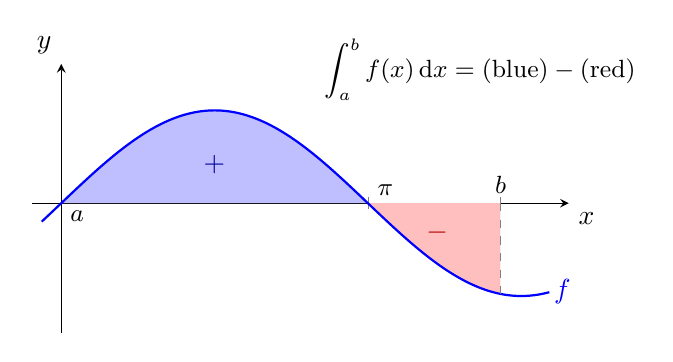
\begin{tikzpicture}
	\begin{axis}[
		axis lines=middle,
		xmin=-0.3, xmax=5.2,
		ymin=-1.4, ymax=1.5,
		xtick={0,3.1416,4.5}, xticklabels={,,},
		ytick=\empty,
		xlabel={$x$}, ylabel={$y$},
		xlabel style={below right}, ylabel style={above left},
		samples=200, smooth, clip=false,
		width=8.4cm, height=5cm
		]
		\addplot[name path=f, thick, blue, domain=-0.2:5] {sin(deg(x))};
		\addplot[name path=axis, draw=none, domain=0:4.5] {0};
		\addplot[blue!25] fill between[of=f and axis, soft clip={domain=0:3.1416}];
		\addplot[red!25] fill between[of=f and axis, soft clip={domain=3.1416:4.5}];
		\node[blue!60!black] at (axis cs:1.57,0.42) {$+$};
		\node[red!70!black] at (axis cs:3.85,-0.32) {$-$};
		\draw[dashed, gray] (axis cs:4.5,0) -- (axis cs:4.5,-0.98);
		\node[anchor=north west, font=\small, inner sep=2pt] at (axis cs:0.03,-0.02) {$a$};
		\node[anchor=south west, font=\small, inner sep=2pt] at (axis cs:3.18,0.02) {$\pi$};
		\node[anchor=south, font=\small, inner sep=2pt] at (axis cs:4.5,0.04) {$b$};
		\node[anchor=south west, font=\small] at (axis cs:2.6,1.0) {$\displaystyle\int_a^b f(x)\,\mathrm{d}x = (\text{blue}) - (\text{red})$};
		\node[blue, anchor=west] at (axis cs:4.95,-0.95) {$f$};
	\end{axis}
\end{tikzpicture}
\end{document}
